%% ------------------------------------------------------------------------- %%
\chapter{Abordagem}
\label{cap:abordagem}

Conforme citado no Capítulo~\ref{cap:fundamentacao-teorica}, uma técnica muito utilizada para a recuperação de trechos de código-fonte é o agrupamento de vetores contínuos ou \textit{joint embedding}. Para utilizar esta técnica, três fatores devem ser levados em consideração:

\begin{itemize}
    \item Representação dos \textit{tokens} ou palavras
    \item Representação das sentenças
    \item Função objetivo do modelo
\end{itemize}

Para a representação das palavras, optamos por uma representação distribuída através do uso do \textit{word2vec} com o algoritmo \textit{skip-gram}, que apresentou um bom desempenho em tarefas semânticas \cite{mikolov2013distributed}. No caso da representação das sentenças, utilizamos redes convolucionais com uma camada de \gls{max-pooling}, priorizando as interações locais e a invariância a pequenas translações (p. ex. alteração da ordem de uma palavra na sentença). Com relação à função objetivo, optamos pela função de perda de articulação ou \textit{hinge loss}, que otimiza a relativa preferência das respostas, ao invés da sua correta classificação.



\section{Representação dos \textit{tokens} ou palavras}
\label{sec:abordagem-representacao-token}

As questões e os trechos de código-fonte são compostos por palavras, pontuações, separadores, caracteres de símbolos e operadores matemáticos. Para as questões, que são descritas em linguagem natural, representamos através de um vetor formado por uma sequência de palavras, apenas removendo os caracteres de acento e pontuação. No caso do código-fonte, acreditamos que os termos presentes no código-fonte contém informações suficientes para estabelecer uma relação semântica entre a questão e o trecho de código-fonte, mesma hipótese utilizada por \citeonline{Sachdev-neural-code-search:2018}. Neste caso, removemos os acentos e caracteres especiais dos trechos de código-fonte, tratando cada termo presente como um \gls{token}.

Uma boa representação para as palavras são os vetores contínuos. De acordo com \citeonline{Goodfellow-et-al-2016}, as redes neurais generalizam bem quando as palavras são representadas através de vetores contínuos. Conforme os próprios autores, uma boa representação deve auxiliar na aprendizagem de uma tarefa posterior. No nosso caso, as representações devem auxiliar o modelo a encontrar uma correlação entre as questões e os trechos de código-fonte mais relevantes.

Mapeamos as palavras para vetores contínuos através do \gls{word2vec} com o algoritmo \gls{skip-gram}, que prediz as palavras do contexto a partir de uma palavra alvo. Segundo \citeonline{mikolov2013distributed}, \textit{skip-gram} obteve um melhor desempenho em problemas semânticos, p .ex., relacionar uma palavra masculina com a equivalente feminina, relacionar o nome de uma capital a um país ou cidade a um estado. No caso do código-fonte, esta é uma característica importante, pois pode auxiliar no agrupamento dos \textit{tokens} por tipo. 

No nosso caso, o \textit{word2vec} mapeou cada palavra para um espaço vetorial $\mathbb{R}^{d}$. Seja $\mathbb{V}$ o conjunto formado pelas palavras das questões e pelas palavras presentes nos trechos de código-fonte. Para cada palavra ${p} \in \mathbb{V}$ temos:

\begin{equation}
    f: {p} \mapsto t_{p},\; t_{p} \in \mathbb{R}^{d}
\end{equation}

Onde $f$ é o \textit{word2vec} com o algoritmo \textit{skip-gram}. A função $f$ mapeia cada palavra pertencente ao vocabulário a uma matriz $\bm{T_{v}}$.
Temos uma matriz $\bm{T}_{v}^{|\mathbb{V}| X d}$, onde $|\mathbb{V}|$ é o tamanho do vocabulário das questões e trechos de código-fonte, e $d$ é a dimensão do vetor contínuo.

Com esta matriz $\bm{T}_{v}$, que contém as palavras das questões e dos trechos de código-fonte mapeadas, podemos representar uma sentença através de vetores contínuos. Dado uma questão $\bm{s} = \{ w_{0}, w_{1}, . . ., w_{n - 1}\}$, onde $w_{i}, 0 \leq i < n$ é uma palavra, podemos representar $\bm{s}$ através de um outro vetor $\bm{x}$, tal que $\bm{x} = \{ x(w_{0}), x(w_{1}), . . ., x(w_{n - 1})\}$, onde $x(w_{i}) \in \bm{T}_{v}$ e $\bm{x}(w_{i}) \in \mathbb{R}^{d}$ é um vetor contínuo. O próximo passo é combinar os elementos do vetor $\bm{x}$ para obter uma representação da sentença.

\section{Representação das sentenças}
\label{sec:representacao-sentenca}

Com cada palavra representada por um vetor contínuo, o próximo passo é combiná-las para obter uma representação para a questão e o trecho de código-fonte. Dado uma sentença $\bm{x} = \{ \bm{x}(0), \bm{x}(1), . . ., \bm{x}(n - 1) \}$, onde $\bm{x}(i) \in \mathbb{R}^{d}$ é um vetor contínuo da $i^{th}$ palavra da sentença e $d$ é a dimensão do vetor. Combinamos os elementos do vetor $\bm{x}$ através de 2 (duas) operações típicas de uma arquitetura CNN:

\begin{itemize}
    \item Operação de convolução
    \item \Gls{max-pooling}
\end{itemize}

A operação de convolução utiliza um filtro $\bm{F}  = [\bm{F}(0),· · ·, \bm{F}(m - 1)]$, tal que $\bm{F} \in \mathbb{R}^{m X d}$. Seja $\bm{x}(i, i + j)$ referência a concatenação dos vetores $\bm{x}(i), \bm{x}(i + 1), . . ., \bm{x}(i + j)$. Ao aplicar $\bm{F}$ em uma janela de \emph{m} palavras $\bm{x}(i, i + m - 1)$, um novo vetor $\bm{c}(i)$ é obtido:

\begin{equation}\label{eq:calc_convolution_ci}
    \bm{c}(i) = tanh \left[\left(\sum_{j=0}^{m - 1} \bm{x}(i + j)^{T}\bm{F}(j)\right) + b\right]
\end{equation}

$\bm{F}$ e $b$ são os parâmetros a serem aprendidos pela rede neural. Para exemplificar esta operação, as Figuras~\ref{fig:first-step-convolutional} e \ref{fig:second-step-convolutional} ilustram um exemplo dos dois primeiros passos da aplicação de um filtro $\bm{F} \in \mathbb{R}^{m X d}$, onde $m = 2$ e $d = 5$. Este filtro é aplicado a uma sentença formado por 6 palavras, que é representada pelo vetor contínuo $\bm{x} \in \mathbb{R}^{n X d}$, onde $n = 6$ e $d = 5$. Pelas figuras, podemos perceber que o parâmetro $m$ do filtro $\bm{F}$ define como as palavras serão combinadas. Nesse caso, foram combinadas de duas em duas, um bi-grama.

\begin{figure}[h]
    \centering
    \caption[Primeiro passo da operação de convolução.]{Primeiro passo da operação de convolução. Aplica-se um filtro $\bm{F} \in \mathbb{R}^{m X d}$, onde $m = 2$ e $d = 5$, em uma sentença $\bm{x} \in \mathbb{R}^{n X d}$, onde $n = 6$ e $d = 5$. Este primeiro passo é equivalente a seguinte operação: $\bm{c}(\bm{0}) = tanh \left[\left(\sum_{j=0}^{m - 1} \bm{x}(\bm{0} + j)^{T}\bm{F}(j)\right) + b\right]$. Figura adapatada a partir do texto de \citeonline{joshua-kim-cnn-understanding-word-embeddings-2019}.}
    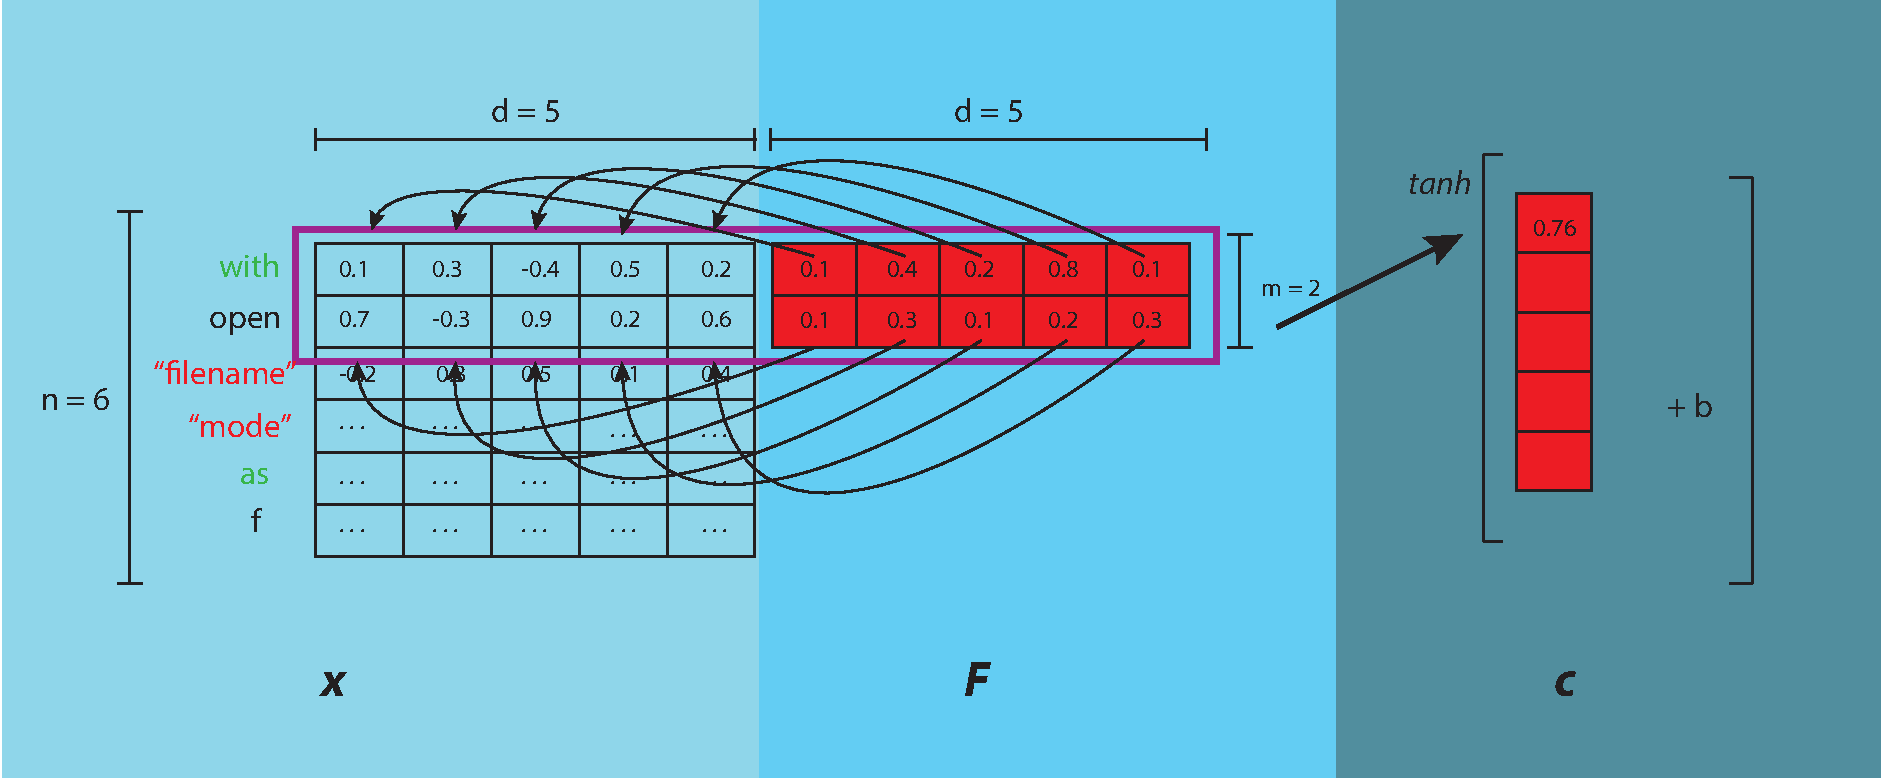
\includegraphics[width=1\textwidth]{figuras/cap-problema/first-step-convolution.pdf}
     \source{Elaborado pelo autor.}
    \label{fig:first-step-convolutional}
\end{figure}

\begin{figure}[h]
    \centering
    \caption[Segundo passo da operação de convolução.]{Segundo passo da operação de convolução. Aplica-se o mesmo filtro $\bm{F} \in \mathbb{R}^{m X d}$ da Figura~\ref{fig:first-step-convolutional}. Neste segundo passo, deslocamos uma posição no eixo $0$. Este segundo passo é equivalente a: $\bm{c}(\bm{1}) = tanh [(\sum_{j=0}^{m - 1} \bm{x}(\bm{1} + j)^{T}\bm{F}(j)) + b]$. Figura adapatada a partir do texto de \citeonline{joshua-kim-cnn-understanding-word-embeddings-2019}.}
    \label{fig:second-step-convolutional}
    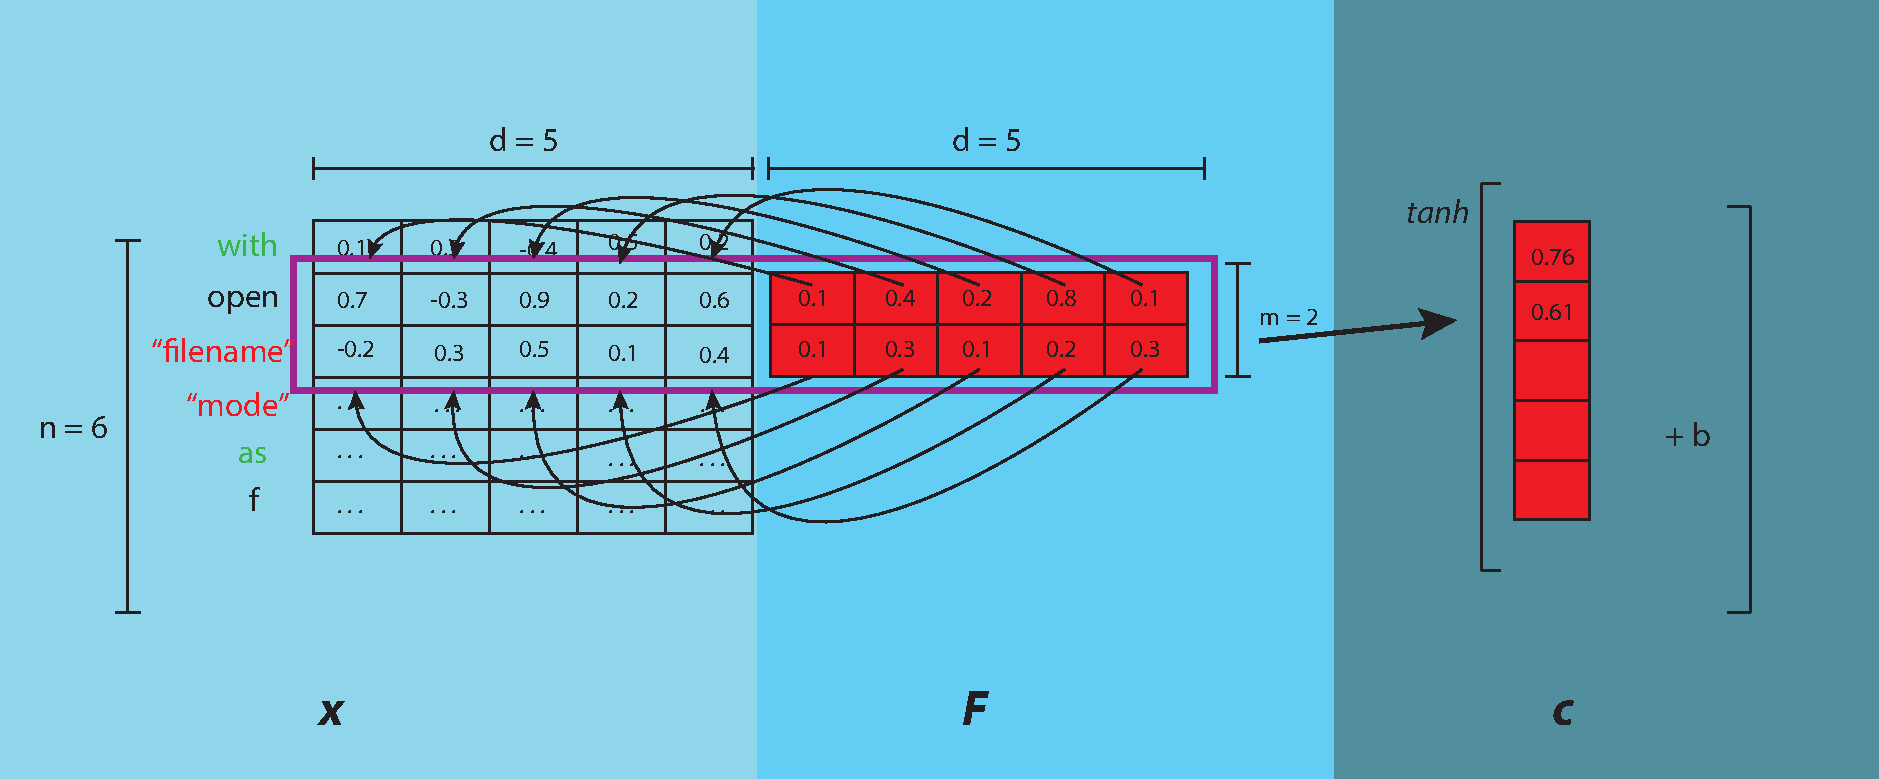
\includegraphics[width=1\textwidth]{figuras/cap-problema/second-step-convolution.pdf}
    \source{Elaborado pelo autor.}
\end{figure}


Durante a operação de convolução, o filtro $\bm{F}$ é aplicado a todas possíveis janelas de palavras utilizando os mesmos pesos para produzir um mapa das características (\textit{feature map}):

\begin{equation}
\label{eq:feature-map}
    \bm{c} = \{ \bm{c}(0), \bm{c}(1), . . ., \bm{c}(n - m) \} 
\end{equation}




Após a operação de convolução, aplicamos a camada \gls{max-pooling}, que reduz a dimensionalidade do vetor $\bm{c}$ através da operação \textit{max}. A operação \textit{max} obtém o maior elemento de um vetor ao longo de um eixo, conforme ilustra a Figura~\ref{fig:cnn-architecture-proposal}. Após esta operação, obtemos o vetor final $\bm{o}$:

\begin{equation}
    \bm{o} = max\left(\left[\bm{c}_{1}, \bm{c}_{2}, . . ., \bm{c}_{|F|}\right], axis = 0\right)
\end{equation}

Para exemplificar a operação completa, a Figura~\ref{fig:cnn-architecture-proposal} ilustra um exemplo da aplicação de 4 filtros em uma sentença de 6 palavras. A sentença é representada através de um vetor $\bm{x} \in \mathbb{R}^{n X d}$, onde $n = 6$ e $d = 5$. Cada filtro $\bm{F} \in \mathbb{R}^{m x d}$ tem dimensão $d = 5$ e janela de tamanho $m = 2$. No nosso trabalho, utilizamos o vetor $\bm{o}$ como o vetor de representação final da nossa sentença. No nosso caso, a sentença pode ser tanto uma questão quanto um trecho de código-fonte. O próximo passo é definir uma função objetivo para ensinar o nosso modelo a discriminar as respostas corretas das incorretas.

\begin{figure}[h]
    \centering
    \caption[Ilustração das 2 operações realizadas pela arquitetura CNN para obter o vetor de representação final $\bm{o}$.]{Ilustração das 2 operações realizadas pela arquitetura CNN para obter o vetor de representação final $\bm{o}$. Neste exemplo, utilizamos 4 filtros $\bm{F} \in \mathbb{R}^{m X d X f}$ com janela de tamanho $m = 2$. Cada filtro é aplicado a sentença $\bm{x} \in \mathbb{R}^{n X d}$, onde $n = 6$ e $d = 5$. }
    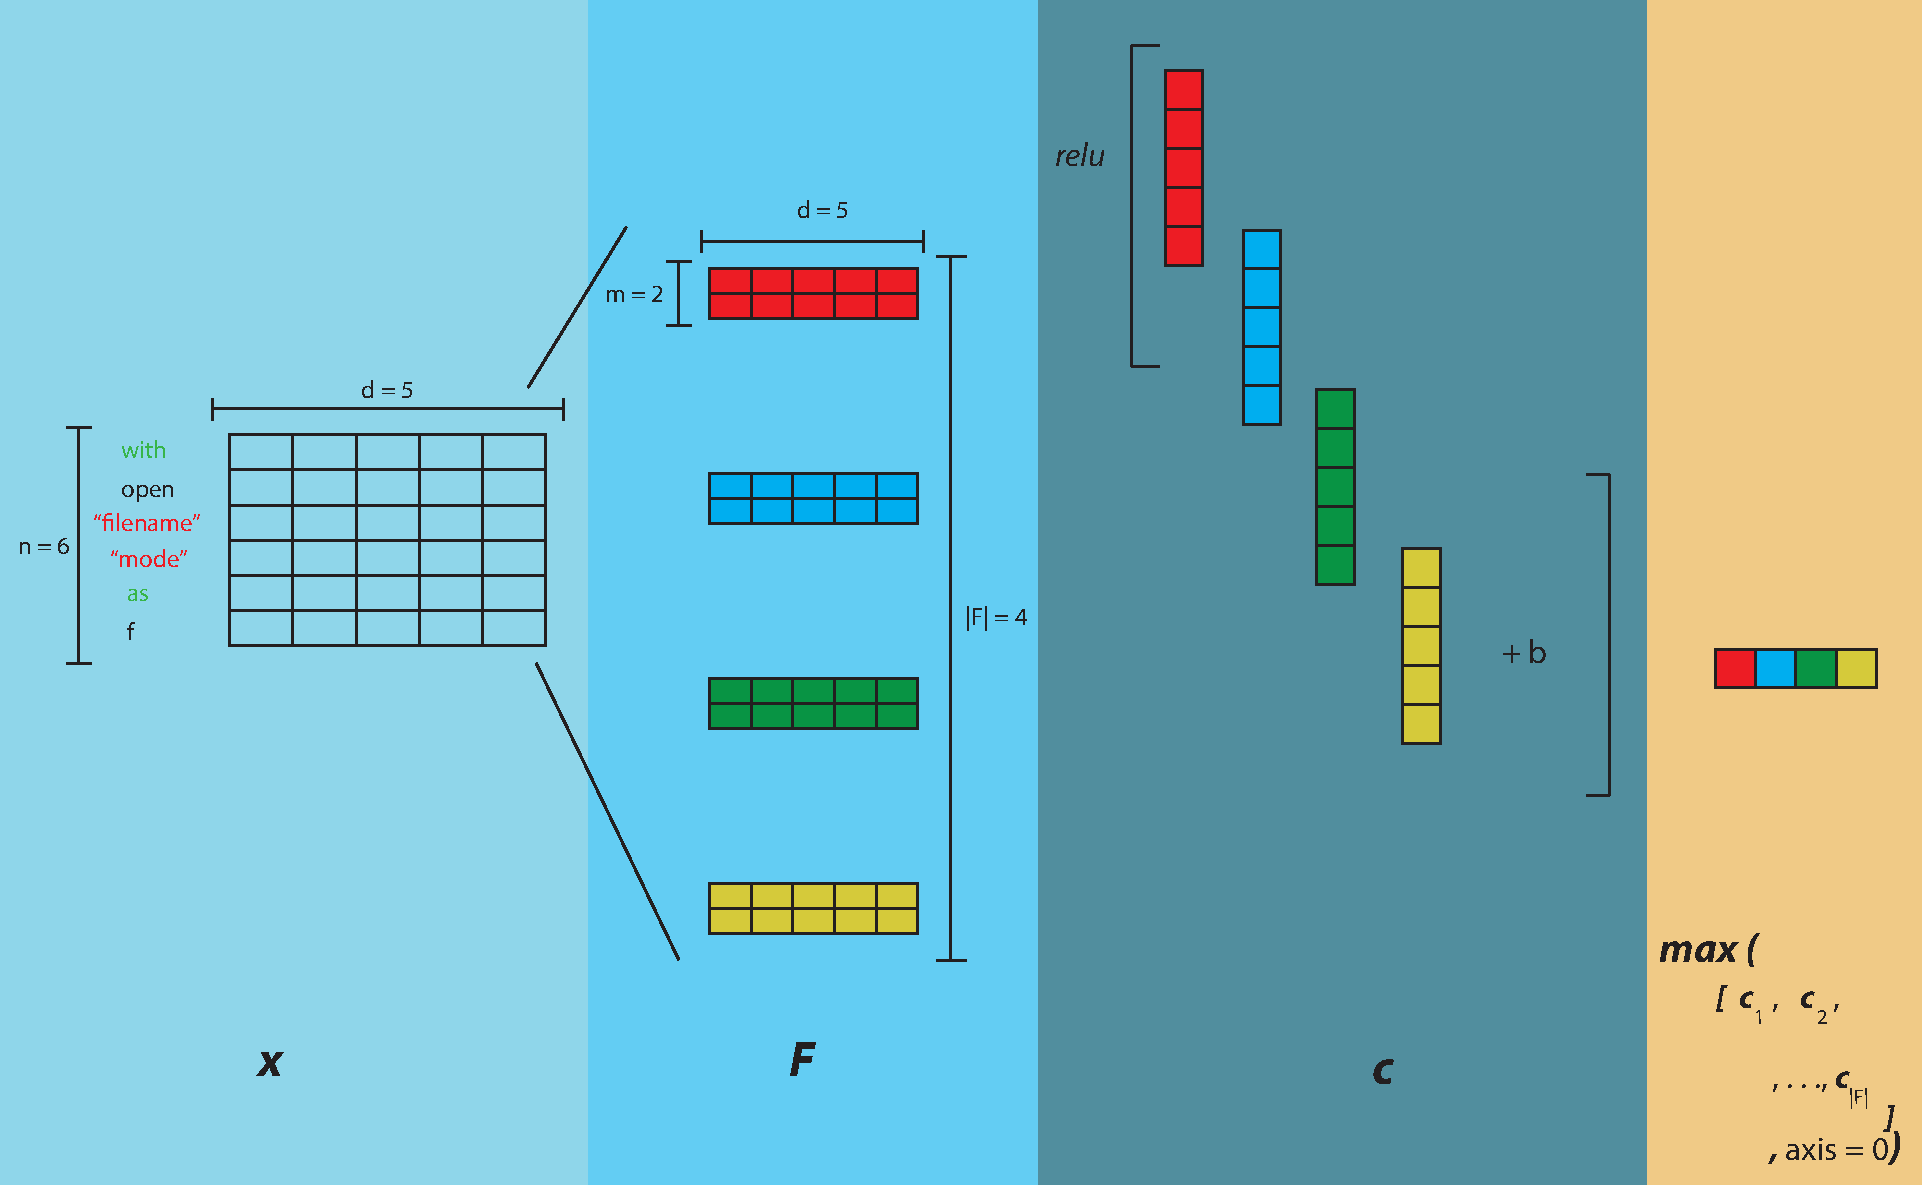
\includegraphics[width=1\textwidth]{figuras/cap-problema/cnn-steps-word-embedding-article.pdf}
    \source{Figura do artigo \citeonline{martins2020concra}.}
    \label{fig:cnn-architecture-proposal}
\end{figure}




\section{Função objetivo}
\label{sec:funcao-objetivo}

O nosso objetivo é ensinar o modelo a classificar os trechos de código anotados como corretos entre as primeiras posições de uma lista. Para isso, adotamos a função de comparação em pares ou \textit{pairwise}, que calcula a relativa preferência dos itens, ao invés da sua correta classificação. Seja $\mathbb{Q}$ um conjunto de questões e $\mathbb{C}$ um conjunto dos trechos de código-fonte. Dado uma tripla $<\bm{q}, \bm{c^{+}}, \bm{c^{-}}>$, onde $\bm{q}$ 
é uma questão, $\bm{c^{+}} \in \mathbb{C}$ é uma resposta anotada como correta e $\bm{c^{-}} \in \mathbb{C}$ é uma resposta incorreta, o objetivo é induzir o modelo a classificar $\bm{c^{+}}$ com uma pontuação maior que $\bm{c^{-}}$. Neste caso, utilizamos função de custo de perda de articulação ou \textit{hinge loss} \cite{feng-2015}:

\begin{equation}
J = max(0, m - h_{\theta}(\bm{q}, \bm{c^{+}}) + h_{\theta}(\bm{q}, \bm{c^{-}}))
\end{equation}

Onde $m$ é uma margem e $h_{\theta}$ é uma função de similaridade, p. ex., \textit{cosine}. Lembrando que o objetivo em uma rede neural é minimizar a função custo $J$. Desta maneira, o modelo vai ser incentivado a satisfazer a seguinte condição: $h_{\theta}(\bm{q}, \bm{c^{+}}) - h_{\theta}(\bm{q}, \bm{c^{-}}) \geq m$. Quer dizer, a função \textit{hinge} induz o modelo a classificar as respostas corretas com uma pontuação maior do que as incorretas por uma certa margem $m$. 



